\section{Methods}\label{methods}

\subsection{Hardware}
<<<<<<< HEAD
Our Hardware consists out of five major parts that are needed to :
-the glasses
The glasses are made out of transparent plastic and have no glasses (?) because their only aim is to 'carry' and stabilize the fixed webcam and the four IR-Markers.

-the illumination
Our illumination source is a IR-Lamp that consists out of 15 IR-LEDs (wvelength? other parameters?). To light up the whole head we placed the lamp approximately 30cm in front of the person.

-the IR-Markers
The IR-Markers consist basically of IR-LEDs (wavelength?, other parameters?) that are powered (over a serial resistor) parallel by a 9V-battery. Each LED is placed in front of ~30cm cables that allows a universal placement. 

-the eye-webcam 
(->Parameter, vl. beschreibe kurz wie der IR-Filter entfernt wurde)

-the notebook with a built-in-webcam 
(-> vl. Mindestanforderungen, bessere Beschreibung?)

(--> Bildchen?)
=======
\begin{figure}[H]
  \centering
  \subfigure[IR light source]{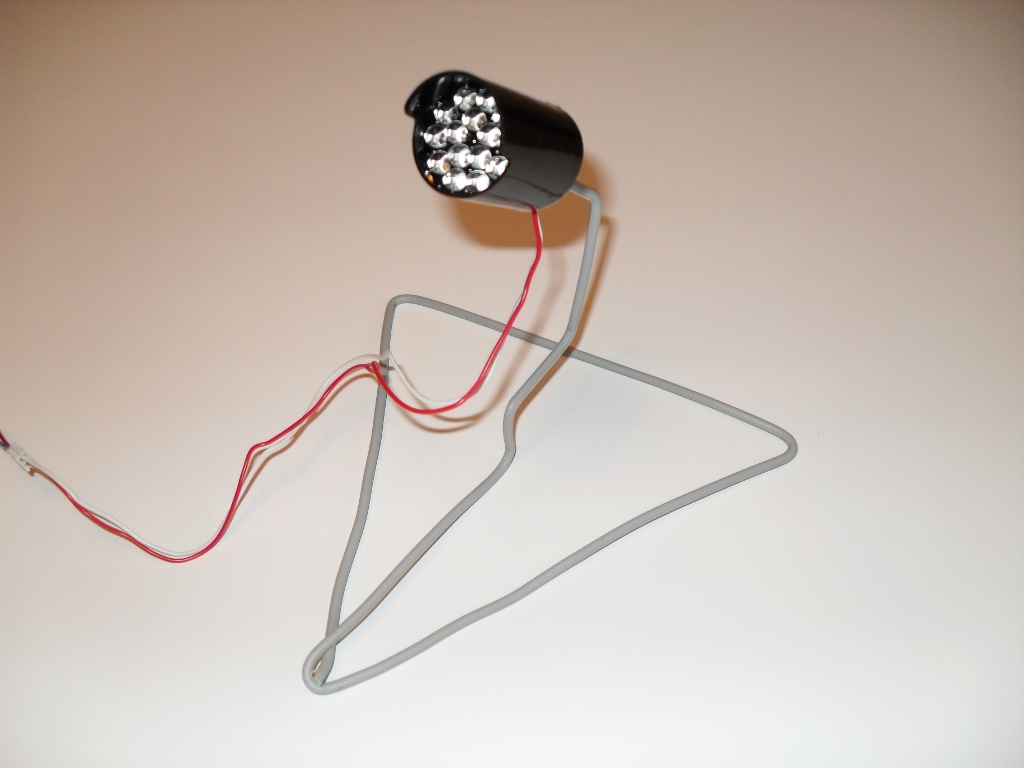
\includegraphics[width=0.4\textwidth]{../finalpres/SDC11117.JPG}}
  \subfigure[Glasses: Front view]{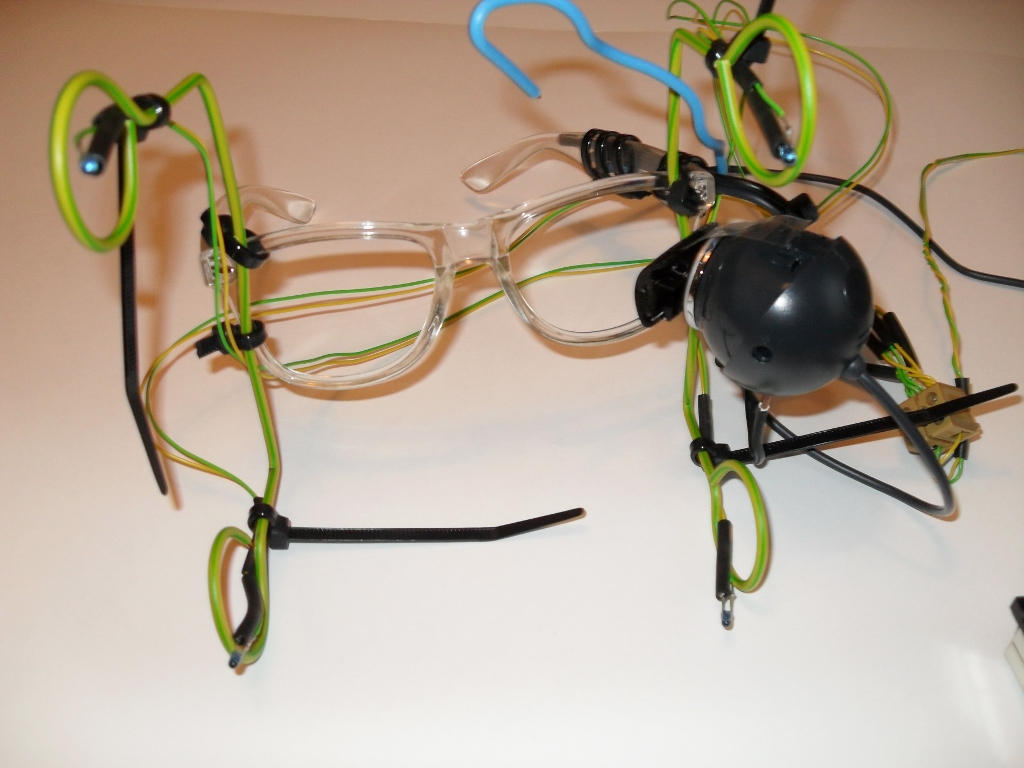
\includegraphics[width=0.4\textwidth]{../finalpres/SDC11119.JPG}}
  \subfigure[Glasses: View from above]{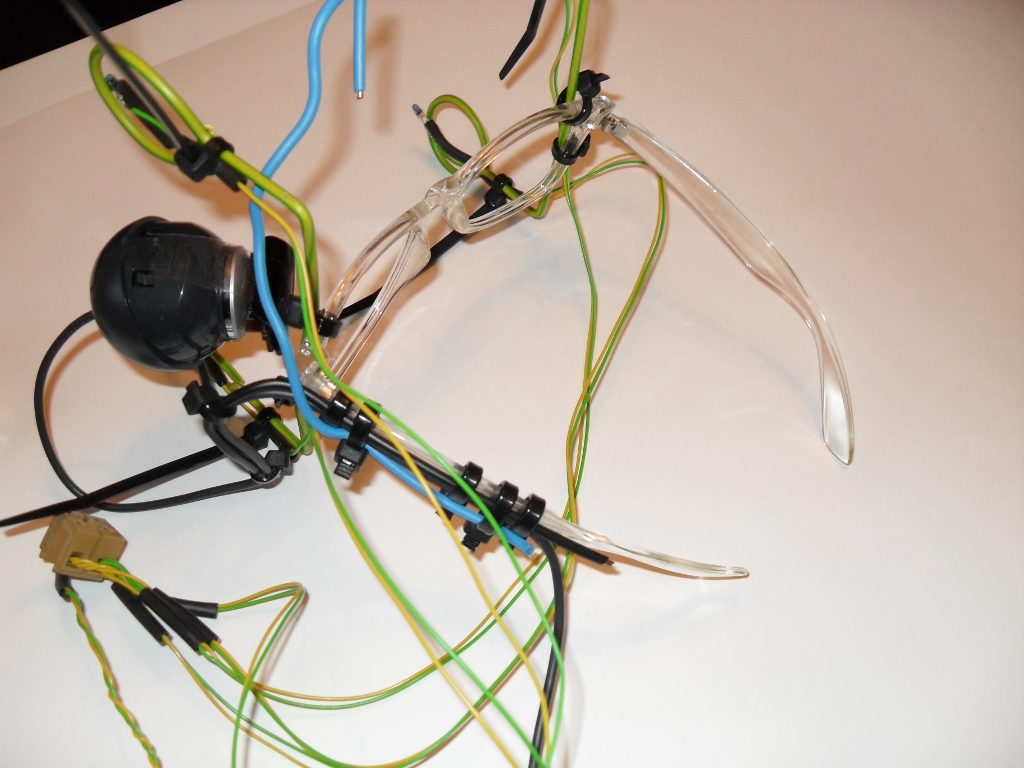
\includegraphics[width=0.4\textwidth]{../finalpres/SDC11121.JPG}}
  \subfigure[Glasses: Another view! Yey!]{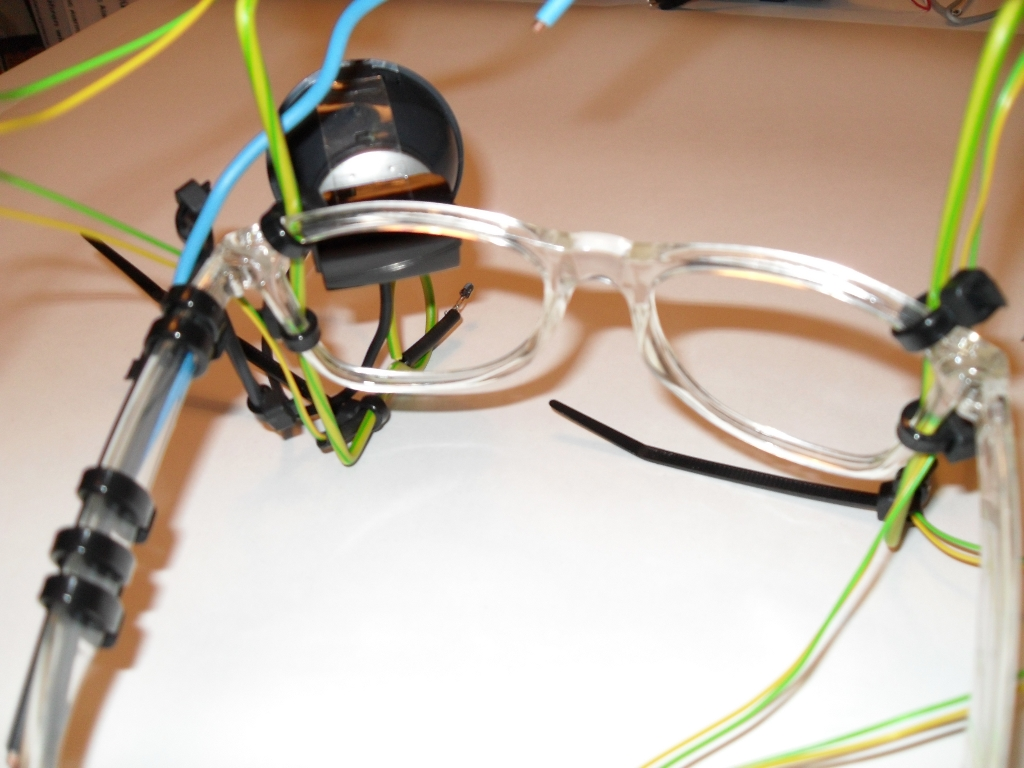
\includegraphics[width=0.4\textwidth]{../finalpres/SDC11122.JPG}}
  \caption{Hardware setup}\label{fig:hardware}
\end{figure}
>>>>>>> bc058c70b7ddbfc8ba70c687a9c68c02da618867

\subsection{Software}

\subsubsection{Basic Principle}
\begin{figure}[H]
  \centering
  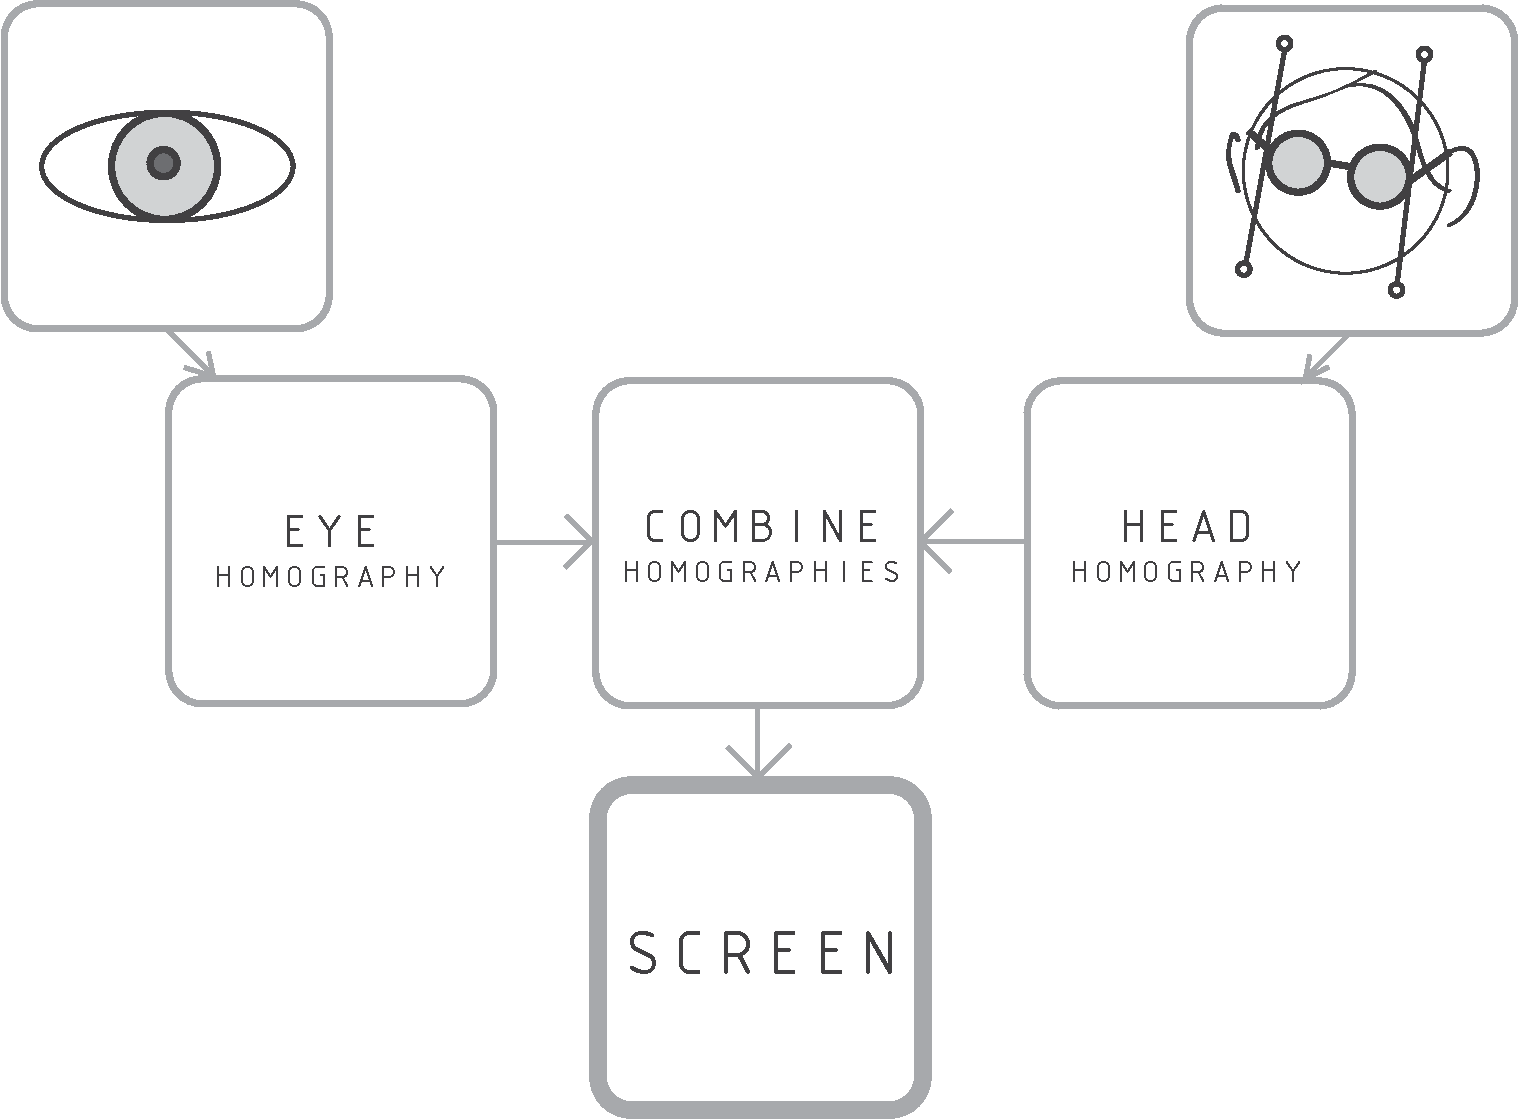
\includegraphics[width=0.9\textwidth]{../finalpres/01c.pdf}
  \caption{Basic principle of the mapping process}\label{fig:basic}
\end{figure}
The primary part necessary for proper mapping is the estimation of the homography. 
This is achieved with a calibration routine. The user has to look at certain defined points on the screen. 
At every point the position of the pupil is determined. 
This information is then used to compute the homography from the pupil position to the screen using the RANSAC algorithm implemented in OpenCV. 

TODO: Head Tracking, Images, Graphics

\subsubsection{Tracking of the pupil}
\begin{figure}[H]
  \centering
  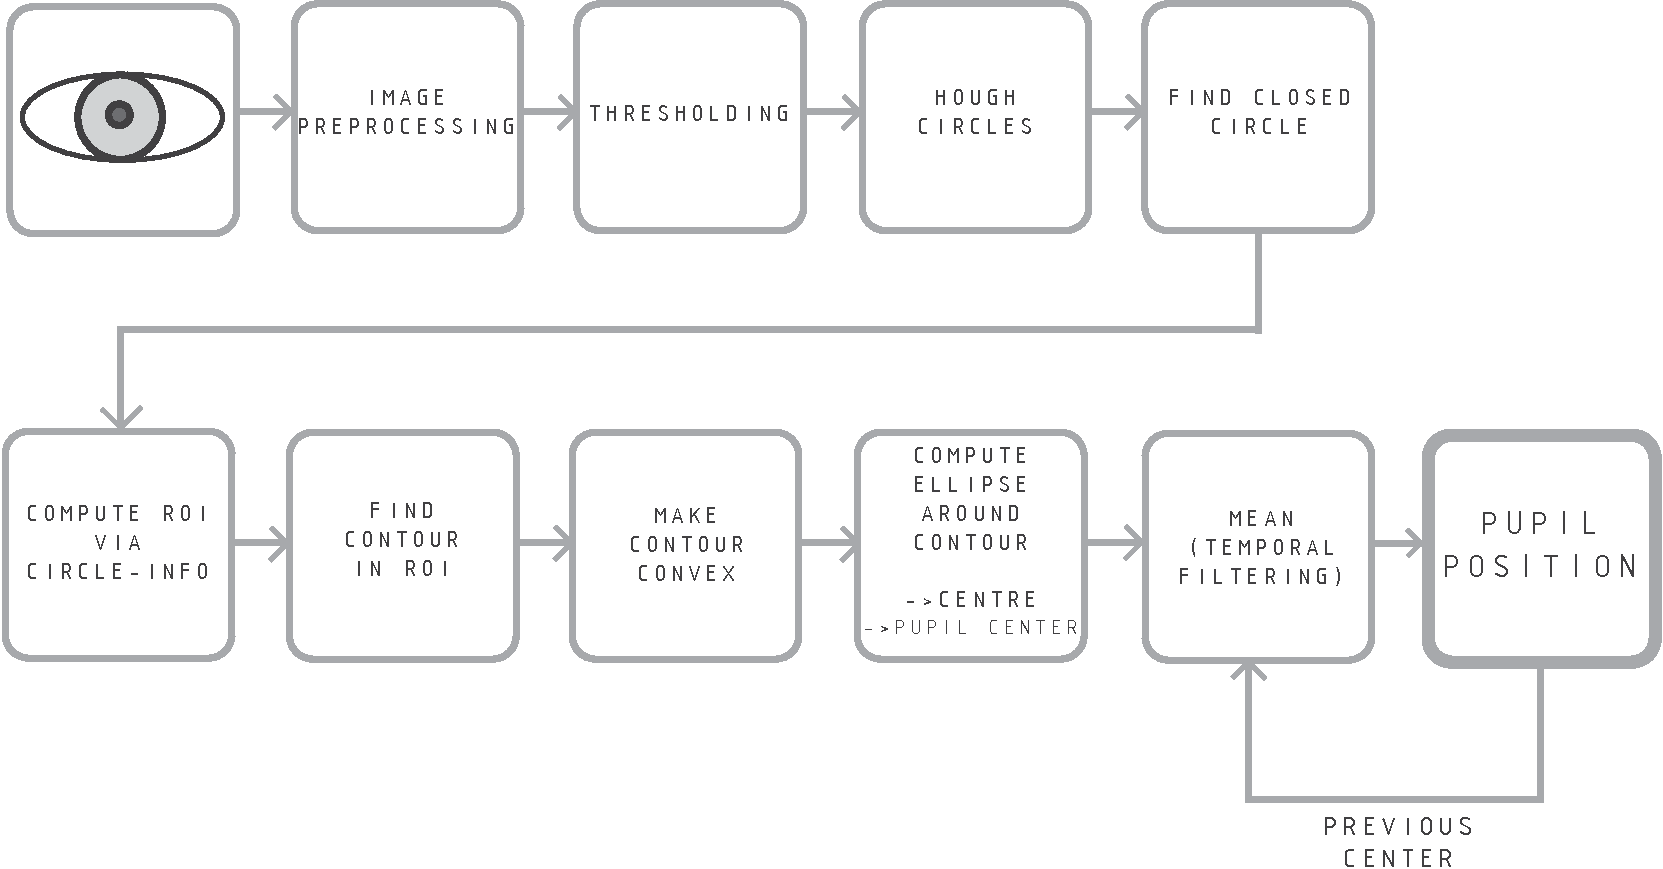
\includegraphics[width=0.9\textwidth]{../finalpres/02c.pdf}
  \caption{Pupil tracking}\label{fig:pupil}
\end{figure}
The first step is to perform several image preprocessing steps on the image aquired by the eye camera. First, the image is converted into the YCrCb color space.
For all the following steps only the Y-Channel is used, as this channel holds the most important information of the captured frame.
On this channel histogram equalization is performed to increase the contrast. 
Eroding the luminance image removes small reflections of the infrared LEDs on the pupil. 
A Gaussian blurring filter takes care of noise in the current frame. 

To segment the pupil from the background, tresholding on the preprocessed image is performed. 
The segmented image is then passed to the OpenCV function \texttt{HoughCircles()}. 
Several restrictions are passed to this function as well in order to assure that no false positives occur. 
In case more than one circle is found, the closest to the previous position gets chosen as next pupil center.
The center found by the \texttt{HoughCircles()} function is not very robust and is therefore not suited to represent the center of the pupil for the tracking process.
Therefore, the information of the Hough space is only used to define a region of interest around the pupil. 
Within this ROI the contour around the pupil is computed by \texttt{findContours()}. 
The function \texttt{convexHull()} returns the convex hull around the pupil, since in some frames, reflections in the pupil cause the contour to be non-convex.
The final step is to fit an ellipse around the contour points (\texttt{fitEllipse()}).
The center of the ellipse is the center of the pupil in the current frame. 
This turns out to perform very well. 

To further smooth the tracking, temporal filtering by computing the mean of the center of the current frame with the center of the previous frame is performed as well. 
Although this slows down the tracking a bit, it is still fast enough for normal use.

\subsubsection{Tracking of the head}
\begin{figure}[H]
  \centering
  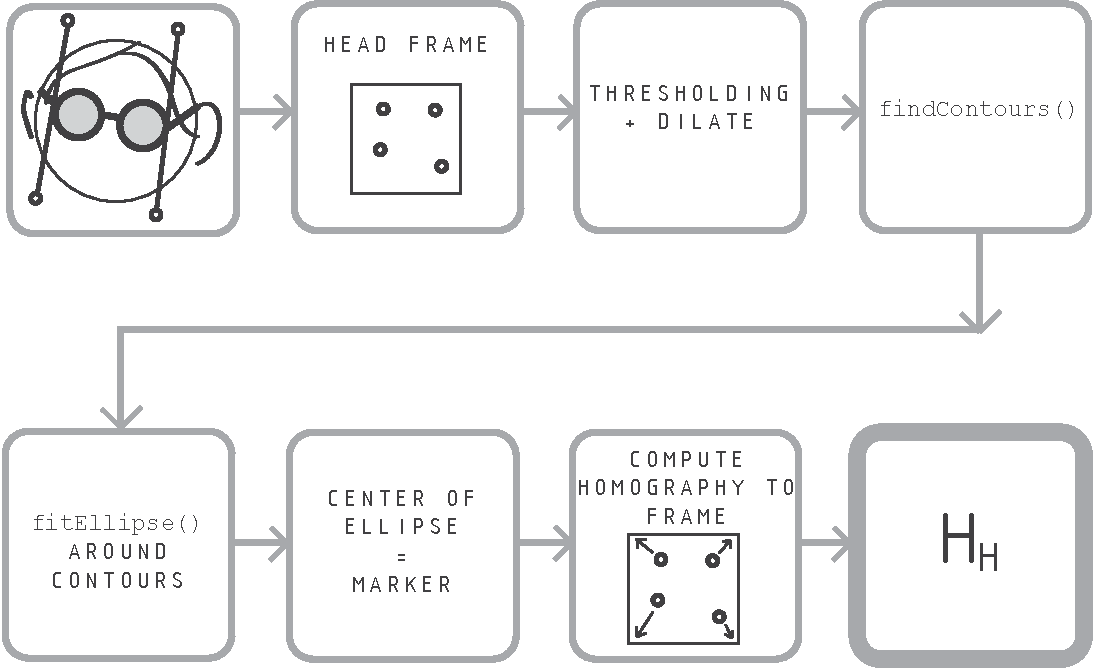
\includegraphics[width=0.9\textwidth]{../finalpres/03c.pdf}
  \caption{Head tracking}\label{fig:head}
\end{figure}

%\begin{Verbatim}[numbers=left,fontsize=\small]
  %CODE
%\end{Verbatim}
